\documentclass[../main.tex]{subfiles}

\begin{document}

Chương này sẽ định nghĩa một cách rõ ràng hơn bài toán nhận diện tên thực thể Y Sinh. Giả sử được cho một văn bản về Y Sinh, ta giả định rằng văn bản này đã được tách từ một cách hoàn chỉnh và biên giữa các câu cũng được định nghĩa đầy đủ. Nhận thấy rằng tên thực thể thường không mở rộng sang 2 câu, ta xem bài toán nhận diện tên thực thể trong văn bản thành nhận diện tên thực thể trong câu. Bài toán chỉ tập trung những thực thể được thể hiện rõ ràng trong câu thay vì tập trung vào cả những thực thể đã được nhắc đến và xuất hiện trong câu hiện tại dưới dạng đại từ. Khi gặp những từ như thế, bài toán sẽ bỏ qua.

Với những giả sử như vậy, mỗi câu $S$ có $n$ từ. Chuỗi từ này được định nghĩa là $S  = {x_{1}, x_{2}, ..., x_{n}}$. Về căn bản, bài toán có thể chia ra làm hai bước: Phát hiện biên của tên thực thể và phân loại tên các thực thể đó. Bước phát hiện biên của thực thể giúp xác định rằng tên thực thể này chỉ bao gồm 1 từ hay gồm nhiều từ. Nói cách khác, việc này giúp xác định tên thực thể với những từ không phải tên thực thể. Bước tiếp theo sẽ gán loại thực thể tương ứng với tên thực thể đã xác định ở bước đầu tiên. Thực thế 2 bước này có thể gộp vào 1 trong mô hình học máy. 

Để giải quyết những vấn đề trên, bài toán nhận diện tên thực thể thường được đưa về bài toán gán nhãn chuỗi. Khi đó, mỗi từ trong một chuỗi sẽ được gán tương ứng với một nhãn thể hiện từ đó có là một phần trong tên của một thực thể nào không.  
Có tập nhãn thường được dùng là BIO hoặc BIOES. Mỗi kí tự là một nhãn thể hiện sự:

- B (Begin):  bắt đầu xuất hiện tên thực thể

- I (Inside): từ nằm trong tên của một thực thể khi đi sau B 

- O (Outside): từ không nằm trong tên của một thực thể

- E (End): đánh dấu tên thực thể kết thúc tại đó

- S (Single): từ đó chính là tên đầy đủ của một thực thể

\begin{figure}[h]
\centering
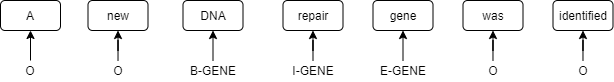
\includegraphics[scale=0.5]{02-sequence-label-example}
\caption{Ví dụ của việc gán nhãn chuỗi với bộ nhãn BIOES}
\end{figure}

Hình 2.1 thể hiện ví dụ của việc gán nhãn chuỗi giúp từ đó xác định tên thực thể. Việc gán nhãn như vậy sẽ vừa giúp xác định được tên của thực thể gồm những từ nào tạo nên, ví trí bắt đầu và kết thúc, cũng như loại thực thể được xác định.

Về tổng quát, có thể mô tả bài toán nhận diện tên thực thể như sau:

Cho $L$ là tập các nhãn thể hiện một từ có thuộc về tên một thực thể hay không. Cho chuỗi các từ $w = \{w_{1}, w_{2}, ..., w_{n}\}$. Đầu ra của bài toán là chuỗi nhãn $y = \{y_{1}, y_{2}, ..., y_{n}\}$ với $y_{i} \in L$


\end{document}